\chapter{Dissociation of Polar Bonds in the Gas Phase and in Solution: A Valence Bond Approach}
\footnotetext{Partly published in ``On the Interpretation of Valence Bond Wavefunctions'', \mbox{R. W. A. Havenith}, \mbox{J. H. van Lenthe}, \mbox{L. W. Jenneskens} and \mbox{J. J. Engelberts}, \textit{Faraday Discuss.} \textbf{2007}, \textsl{135}, 299-308.}
\label{chap_dissociation}

\hyphenation{chlo-ro-me-thane pro-noun-ced mol-e-cules}

\ifthenelse{\boolean{wholethesis}}{\relax}{\begin{center}\textit{Generated on \today\ at \currenttime}\end{center}}

\noindent\textbf{Abstract:} The influence of a solvent on the dissociation behavior of four chlorine containing compounds with varying polarity, chloromethane, \textit{tert}-butylchloride, chlorosilane and trimethylsilylchloride, is analyzed with VB in conjunction with the Polarizable Continuum Model (PCM), in which the solvent is represented as a homogeneous medium that is characterized by its dielectric constant. VB calculations without solvent effects show that all four molecules dissociate to a radical chlorine atom and an alkyl/silyl radical. When water as a solvent is mimicked by PCM \textit{tert}-butylchloride, chlorosilane and trimethylsilylchloride dissociate to ions, whereas chloromethane is hardly influenced by the solvating medium. Homolytic bond dissociation to radicals occurs.

In the last part of this chapter it is shown that the C--H orbitals, albeit separated by one bond from the active center, are involved in the reaction via hyperconjugation which stabilizes the \textit{tert}-butyl cation. 

\clearpage

\section{Introduction}

\lettrine{\initial{C}}{}hemical bonds can be classified into several categories, like covalent (polar and apolar), ionic, and metallic bonds. An apolar covalent bond is a chemical bond, in which atoms share equally electrons in order to obtain a noble gas configuration. An example is H$_2$ (Figure \ref{ch3.fig.h_twee}), where each hydrogen atom contributes one electron to the bond, resulting in a noble gas configuration (He) for both of them.
\begin{figure}[ht]
\center
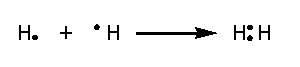
\includegraphics{dissociation/figures/h_twee.eps}
\caption{Two hydrogen atoms forming a H$_2$ molecule (Lewis structure on the right).}
\label{ch3.fig.h_twee} 
\end{figure}

If one electron is transferred from one atom to the other, which results in two oppositely charged ions, the bond is completely ionic, as in \textit{e.g.} NaCl (Figure \ref{ch3.fig.nacl}). The ions remain bound only by electrostatic interactions. 
\begin{figure}[ht]
\center
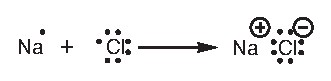
\includegraphics{dissociation/figures/nacl.eps}
\caption{A sodium and a chlorine atom forming a NaCl ``molecule''.}
\label{ch3.fig.nacl}
\end{figure}

In between these two extremes is the polar bond, which possesses mixed covalent and ionic character. Hydrogenchloride (HCl) is such a molecule (Figure \ref{ch3.fig.hcl}). Although hydrogen and chlorine share electrons the electron pair will be located more on the chlorine than on the hydrogen atom, due to the higher electronegativity of chlorine.
\begin{figure}[ht]
\center
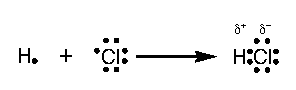
\includegraphics{dissociation/figures/hcl.eps}
\caption{A hydrogen and a chlorine atom forming a HCl molecule.}
\label{ch3.fig.hcl}
\end{figure}

Shaik \textit{et al.} have defined a fourth bond type, the charge-shift bond \cite{cs1,cs2}. They define this bond as a fundamental bond type for those electron pair bonds that are neither covalent, nor ionic in nature. Characteristics for charge-shift bonds are a large charge-shift resonance energy ($RE_{CS}$) and a relatively small contribution of the covalent structure ($D_\mathrm{cov}$). It is, however, not limited to molecules that can be considered as ``in between'' covalent and ionic in nature. The bond in fluorine (F$_2$, Figure \ref{ch3.fig.f_twee}), a homopolar, homonuclear diatomic molecule, is classified as a charge-shift bond.
\begin{figure}[h]
\center
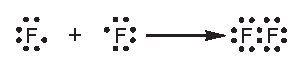
\includegraphics{dissociation/figures/f_twee.eps}
\caption{Two fluorine atoms forming a F$_2$ molecule.}
\label{ch3.fig.f_twee} 
\end{figure}

In this chapter, the dissociation of polar bonds is studied with the Valence Bond method, in which the wave function can be expressed in covalent and ionic structures. In reference \cite{interpret} a discussion on the assumed equivalence of Lewis and Valence Bond structures is presented. As an introduction dissociation curves for H$_2$ (covalent bond), the ``NaCl'' molecule (ionic bond) and F$_2$ (charge-shift bond) in the gas phase are presented to show the differences in dissocation of these chemical bonds.

The central question in this chapter is: How does the dissociation change when the parameters influencing the bond, like the atoms involved, the surrounding medium and different functional groups, are changed?

To obtain answers to this question, the dissociation pathway of several polar bonds with different polarity and in different media, \textit{viz.} vacuum and water, will be studied.  The set of molecules consists of chloromethane (\textbf{1}), which possesses a typical polar C--Cl bond, \textit{tert}-butylchloride (\textbf{2}) and their silicon analogues chlorosilane (\textbf{3}) and trimethylsilylchloride (\textbf{4}) (Figure \ref{ch3.fig.compounds}).  
\begin{figure}[htbp]
\begin{center}
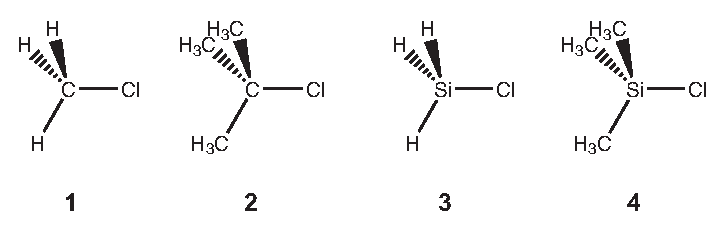
\includegraphics{dissociation/figures/compounds.eps}
\end{center}
\caption{Chloromethane (CH$_3$Cl, \textbf{1}), \textit{tert}-butylchloride
(C(CH$_3$)$_3$Cl, \textbf{2}), chlorosilane (SiH$_3$Cl, \textbf{3}) and trimethylsilanechloride
(Si(CH$_3$)$_3$Cl, \textbf{4})}
\label{ch3.fig.compounds}
\end{figure} 
The bond that will be broken is the C/Si--Cl bond. The silicon analogues have been selected because silicon has a much lower electronegativity than carbon (compare the Pauling electronegativity of 1.90 for silicon with 2.55 for carbon \cite{handbook}). The influence this difference may have on the dissociation behavior of carbon and silicon compounds is analyzed. Furthermore, the influence of the difference between hydrogen atoms and methyl-groups on the dissocation will be compared. Methyl-groups exert an electron donating character \cite{mcmurry}, compared to hydrogen. Besides, the methyl-hydrogens might exert an effect on the dissociation process through hyperconjugation \cite{march}, not present in the hydrogen substituted compounds. Orbitals on the C--H bonds of the methyl-groups, which are several bond lengths separated from the tertiary carbon atom, may still have an influence on it, and hence on the dissociation behavior. 

The alteration of the dissociation behavior by different surrounding media will be investigated using calculations performed with the Polarizable Continuum Model (PCM) \cite{pcm1,pcm2} which accounts for solvation effects in its simplest form: the solvent is represented as a homogeneous medium that is characterized by its dielectric constant without further explicit molecular interactions between the solvent molecules and the solute. 

The Valence Bond wave functions used to describe the dissociation behavior of these molecules contain the three structures presented in Figure \ref{ch3.fig.structures}.
\begin{figure}[htbp]
\begin{center}
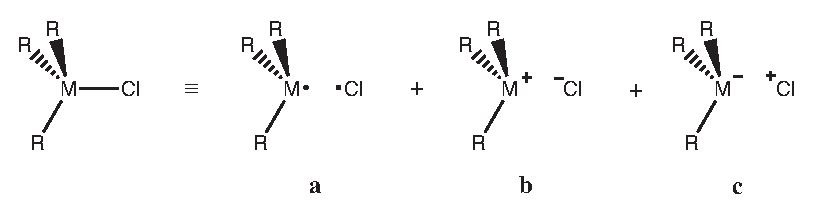
\includegraphics{dissociation/figures/structures.eps}
\end{center}
\caption{The Valence Bond structures, a covalent (\textbf{a}) and two ionic (\textbf{b} and \textbf{c}) structures (M=C or Si; R=H or CH$_3$).}
\label{ch3.fig.structures}
\end{figure}
An indication of the polarity of the bond is given by weights attributed to the structures \cite{coulson}. 

For all four compounds dissociation energies from prior VB calculations are available. Lauvergnat \textit{et al.} \cite{lauvergnat} performed VBSCF \cite{vbscf1,vbscf2} and BOVB \cite{bovb1,bovb2,bovb3} calculations on \textbf{1} and \textbf{3} in the gas phase. They concluded that BOVB is necessary to obtain a dissociation energy that is close to the experimental value (334.3 kJ/mol (BOVB) \textit{vs} 365.3 kJ/mol (experimental) for \textbf{1} and 425.5 kJ/mol (BOVB) \textit{vs} 463.2 kJ/mol (experimental) for \textbf{3}), but that VBSCF calculations sufficed to obtain qualitatively correct results.  Song \textit{et al.} \cite{song} have performed test calculations with VB in conjunction with PCM, to which they refer as VBPCM, on \textit{tert}-butylchloride (\textbf{2}) with frozen C--H bond orbitals. The latter study confirmed the heterolytic dissociation of \textbf{2} in water as a solvent. Su \textit{et al.} \cite{psu} have investigated \textbf{2} and \textbf{4} in the gas phase and with VBPCM. They have concluded that the C--Cl and Si--Cl bonds are of different natures. While C--Cl is considered to be a covalent bond, Su \textit{et al.} consider Si--Cl to be of the category of charge-shift bonds. The reasoning behind this is the significantly higher resonance energy in the silicon case. Our results will further extend the study of the dissociation of polar, \textit{cq.} charge-shift bonds.

The research is split-up in four parts.  In the first part, Valence Bond results of the dissociation of a purely covalent (H$_2$), a purely ionic (NaCl) compound and a charge-shift bond (F$_2$) in the gas phase will be presented to illustrate the differences between these three in dissociation, \textit{i.e.} H$_2$ for covalent, NaCl for ionic and F$_2$ for charge-shift. Secondly, compounds \textbf{1}-\textbf{4} are investigated in the gas phase using Valence Bond theory. Thirdly, the effect of water as a solvent on the dissociation pathways of these compounds is analyzed with PCM. Finally, it will be shown that freezing of orbitals, in particular C--H orbitals, may inadvertently affect the results of the calculation. It is shown that the observed effect is linked to contributions of the phenomenon of hyperconjugation.

\section{Dissociation of H$_2$, NaCl and F$_2$ in the Gas Phase}

In the H$_2$ molecule, both hydrogen atoms contribute one electron to the bond. The two electrons can be arranged in four ways, expressed in the three Lewis structures:
\begin{equation}
\nonumber
\mathrm{H-H\ \ \equiv \ \ H^{\bullet}\ \ H^{\bullet}\ \ +\ \ H^{+}\ \ H^{-}\ \ +\ \ H^{-}\ \ H^{+}}.
\end{equation}
Both electrons can be located on their individual atoms ($\mathrm{H^{\bullet}\ \ H^{\bullet}}$) or both electrons can be located on one of the hydrogen atoms ($\mathrm{H^{+}\ \ H^{-}}$ and $\mathrm{H^{-}\ \ H^{+}}$). To analyze the dissociation of the H$_2$ bond theoretically, it is expressed in the three VB structures:
\begin{equation}
\nonumber
\Psi_{\mathrm{H_2}} = c_1\cdot [\mathrm{H}^\bullet \mathrm{H}^\bullet] + c_2 \cdot [\mathrm{H}^{+}\mathrm{H}^{-}] + c_3 \cdot [\mathrm{H}^{-}\mathrm{H}^{+}]. 
\end{equation}
Energies for the total wave function and the structures separately are calculated at different interatomic distances. Because $[\mathrm{H}^{+}\mathrm{H}^{-}]$ and $[\mathrm{H}^{-}\mathrm{H}^{+}]$ are equivalent their corresponding coefficients will be equal ($c_2 = c_3$).  

In Figure \ref{ch3.fig.h2_c} the dissociation path for H$_2$ is shown. The total energy curve ($E_\mathrm{tot}^\mathrm{gas}$) and the energy curves of the covalent ($E_\mathrm{cov}^\mathrm{gas}$) and ionic ($E_\mathrm{ion}^\mathrm{gas}$) structures separately are presented. 
\begin{figure}[htbp]
\begin{center}
\includegraphics[scale=0.6]{dissociation/figures/h2_g.eps}
\end{center}
\caption{The dissociation curve of H$_2$ in the gas phase. $E_\mathrm{tot}^\mathrm{gas}$ is the total VB energy, $E_\mathrm{cov}^\mathrm{gas}$  and $E_\mathrm{ion}^\mathrm{gas}$ are the energies of the covalent $[\mathrm{H^\bullet H^\bullet}]$ and ionic $[\mathrm{H^{+}H^{-}}]$ structures separately. The minima are shown in parenthesis.}
\label{ch3.fig.h2_c}
\end{figure}
The total and covalent curves practically coincide over the whole range. This indicates the covalent character of the bond in H$_2$. For the covalent structure the weight is at least 0.8 over the whole dissociation range.

Typical for the ionic and covalent curves is that they are easily distinguishable by their shape, at least in the curves presented here. The value of $E_\mathrm{ion}^\mathrm{gas}$ increases with increasing bonding distance from the minimum in energy to higher distances. In the covalent curves the increase in $E_\mathrm{cov}^\mathrm{gas}$ from the minimum in energy going to larger distances stops at distances roughly varying from 2.5 to 4.0 \AA. An explanation for the gradual increase of the ionic curves, not seen in either the covalent or neutral curves, can be found in electrostatics (Coulomb attraction): when two oppositely charged bodies, in this case atoms or molecular fragments, are separated, the potential energy increases inversely proportional to the separation distance ($\frac{1}{r}$).

In analogy with $\Psi_{\mathrm{H_2}}$, a three structure VB wave function for the NaCl ``molecule'' is constructed:
\begin{equation}
\nonumber
\Psi_{\mathrm{NaCl}} = c_1\cdot [\mathrm{Na}^\bullet \mathrm{Cl}^\bullet] + c_2 \cdot [\mathrm{Na}^{+}\mathrm{Cl}^{-}] + c_3 \cdot [\mathrm{Na}^{-}\mathrm{Cl}^{+}]. 
\end{equation}
Dissociation curves for $\Psi_{\mathrm{NaCl}}$ are presented in Figure \ref{ch3.fig.nacl_c}.
\begin{figure}[hbtp]
\begin{center}
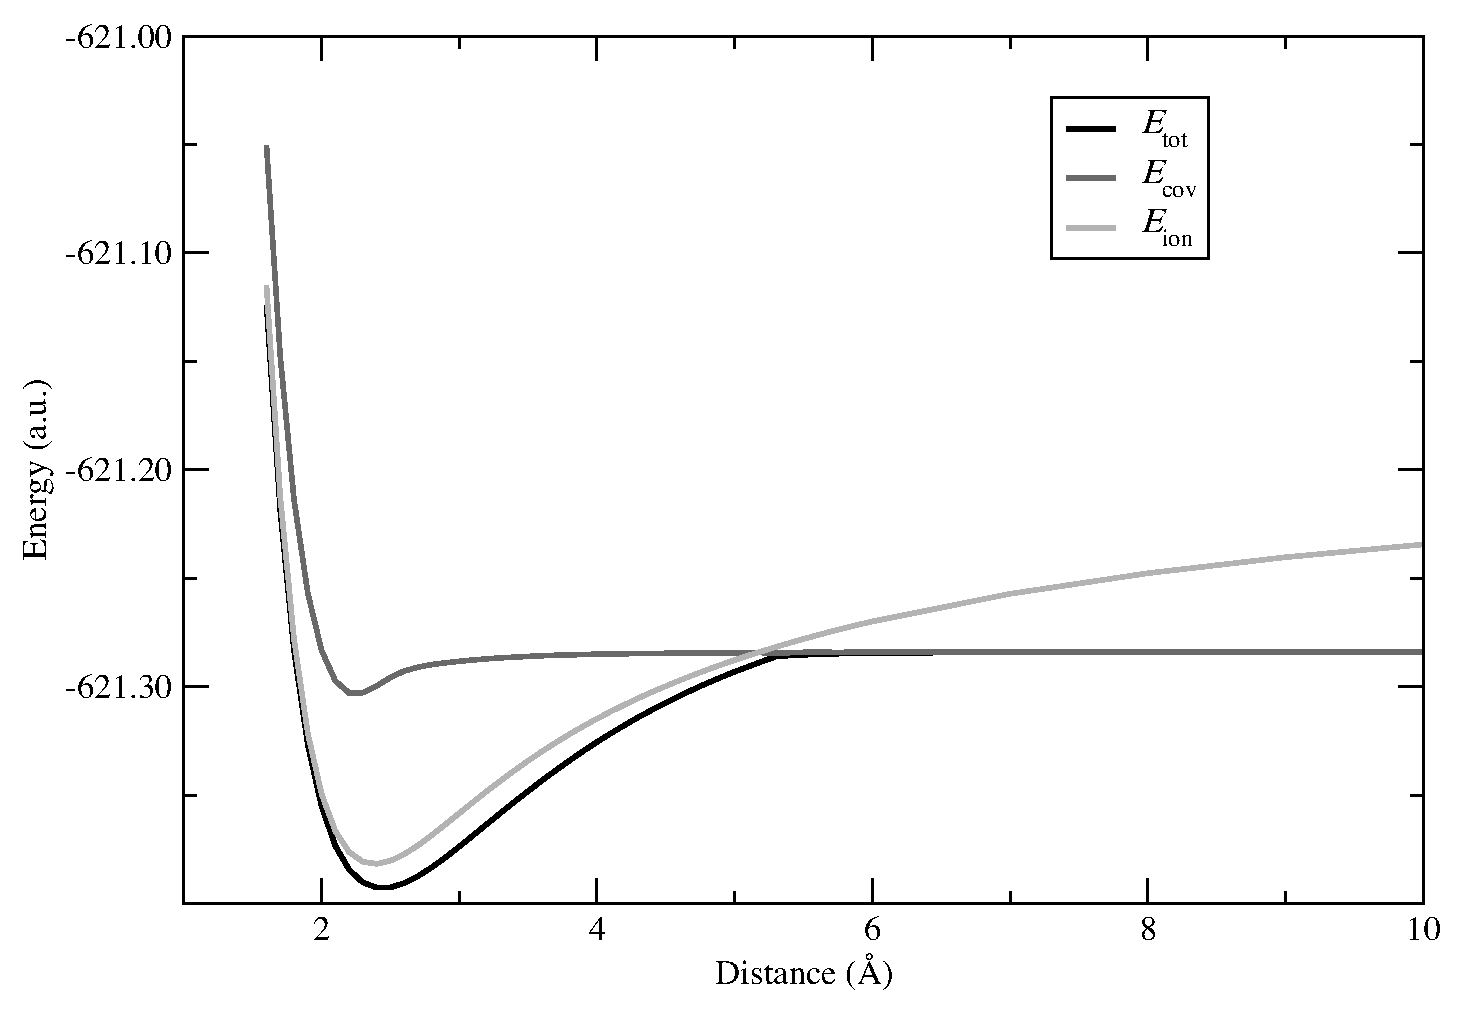
\includegraphics[scale=0.6]{dissociation/figures/nacl_g.eps}
\end{center}
\caption{The dissociation curve of the NaCl ``molecule'' in the gas phase. $E_\mathrm{tot}^\mathrm{gas}$ is the total VB energy, $E_\mathrm{cov}^\mathrm{gas}$  and $E_\mathrm{ion}^\mathrm{gas}$ are the energies of the covalent $[\mathrm{Na^\bullet Cl^\bullet}]$ and ionic $[\mathrm{Na^{+}Cl^{-}}]$ structures separately. The minima are shown in parenthesis.}
\label{ch3.fig.nacl_c}
\end{figure}
The curve for the $[\mathrm{Na}^{-}\mathrm{Cl}^{+}]$ structure has been omitted, because its energy is approximately 0.5 a.u. higher than for the other two structures over the whole range and its contribution to the wave function is negligible ($c_3 \approx 0$). Nevertheless, it is included in $\Psi_{\mathrm{NaCl}}$ to keep the general expression of the wave functions, \textit{i.e.} built from three structures, equal for all molecules in this chapter:
\begin{equation}
\nonumber
\Psi_{\mathrm{AB}} = c_1\cdot [\mathrm{A}^\bullet \mathrm{B}^\bullet] + c_2 \cdot [\mathrm{A}^{+}\mathrm{B}^{-}] 
+ c_3 \cdot [\mathrm{A}^{-}\mathrm{B}^{+}],
\end{equation}
in which $\mathrm{A}$ and $\mathrm{B}$ can be atoms or molecular fragments (structures \textbf{a}, \textbf{b} and \textbf{c} in Figure \ref{ch3.fig.structures}).

Like for the other two molecules, a three structure VB wave function is constructed for F$_2$:
\begin{equation}
\nonumber
\Psi_{\mathrm{F_2}} = c_1\cdot [\mathrm{F}^\bullet \mathrm{F}^\bullet] + c_2 \cdot [\mathrm{F}^{+}\mathrm{F}^{-}] + c_3 \cdot [\mathrm{F}^{-}\mathrm{F}^{+}]. 
\end{equation}
In analogy with H$_2$, the coefficients $c_2$ and $c_3$ are equal. The dissociation curves are presented in \ref{ch3.fig.f2_c}.
\begin{figure}[hbtp]
\begin{center}
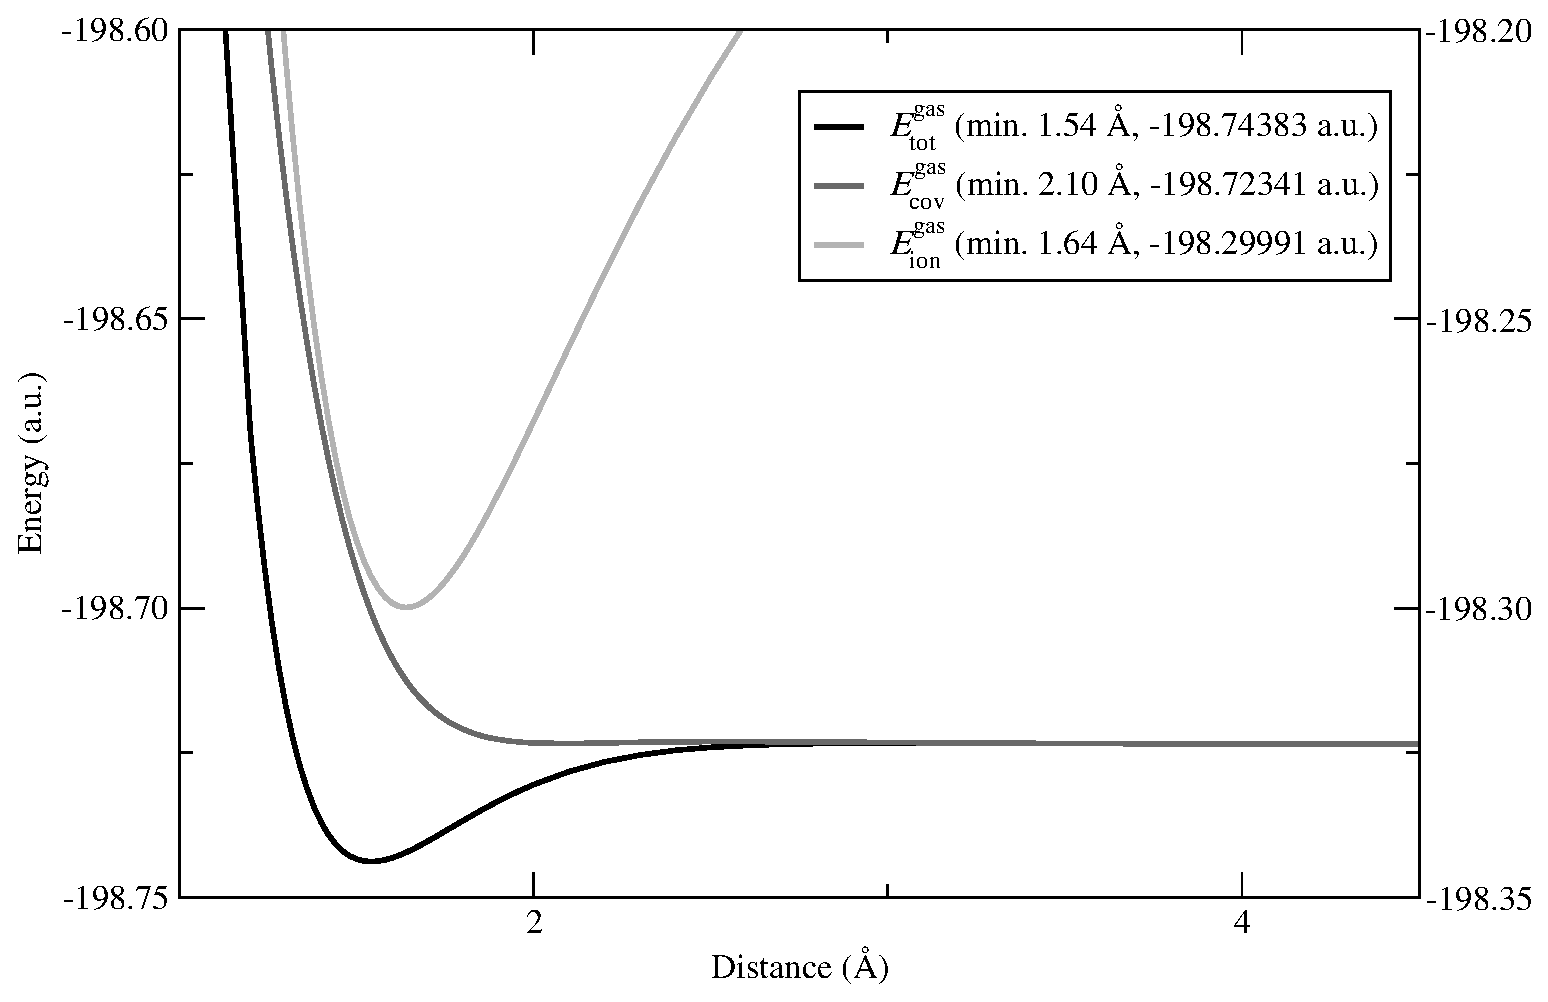
\includegraphics[scale=0.6]{dissociation/figures/f2_g.eps}
\end{center}
\caption{The dissociation curve of F$_2$ in the gas phase. $E_\mathrm{tot}^\mathrm{gas}$ is the total VB energy, $E_\mathrm{cov}^\mathrm{gas}$ is the curve of the covalent $[\mathrm{F^\bullet F^\bullet}]$ structure. The ionic curve with energy $E_\mathrm{ion}^\mathrm{gas}$ of the ionic structure  $[\mathrm{F}^{+}\mathrm{F}^{-}]$ is shifted by 0.4 a.u. to make it visible in the figure. Its energy scale is shown on the right hand side of the graph. The minima are shown in parenthesis.}
\label{ch3.fig.f2_c}
\end{figure}
The curve for the ionic structure ($E_\mathrm{ion}^\mathrm{gas}$) has been shifted by 0.4 a.u. in Figure \ref{ch3.fig.f2_c} because it is lying much higher than the curve for the total energy $E_\mathrm{tot}^\mathrm{gas}$ and hence would not have been visible, otherwise. The energy scale for the ionic structure is shown on the right hand side of the graph.

For H$_2$, the total energy curve coincides with the covalent curve (Figure \ref{ch3.fig.h2_c}), indicating that the covalent VB structure roughly corresponds to the bonding picture. The weight of the structure in the total wave function, as introduced by Chirgwin and Coulson \cite{chirgwin}, is 0.80 around the equilibrium distance. Charge-shift resonance energy, \textit{i.e.} the energy difference between the most stable structure (lowest in energy) and the total energy ($RE_{CS}$ \cite{cs1}), is 0.011 a.u. 

In the case of NaCl, the total energy curve coincides with the ionic curve around the equilibrium distance (Figure \ref{ch3.fig.nacl_c}), indicating that the ionic VB structure roughly corresponds to the bonding picture. This is further corroborated by the weight of the ionic structure at equilibrium distance (0.70) and the low resonance energy (0.025 a.u.).

For F$_2$, the covalent curve is lying much higher in energy than the total energy curve, while the ionic curve is even higher. The latter curve has been shifted by 0.4 a.u. to make its form visible in Figure \ref{ch3.fig.f2_c}. The covalent curve is lying above the energy level for two separate fluorine radicals and hence the covalent structure is non bonding in itself. Neither the covalent, nor the ionic structure represents the bonding, but rather the combination of the two does. Although the weight for the covalent structure is rather high (0.84) like for H$_2$, the high resonance energy (0.047) compared to H$_2$ suggests that the bond is rather different than a typical covalent bond. Shaik \textit{et al.} therefore classify this bond as of the charge-shift type \cite{cs1,cs2}.

An important difference between the curves of H$_2$ and NaCl is that in the latter case the covalent and ionic curves cross. At infinite distance the atoms Na and Cl are neutral, both having an odd number of electrons (Na 11 and Cl 17). There, the covalent description prevails, characterized by the coincidence of the $E_\mathrm{tot}^\mathrm{gas}$ and $E_\mathrm{cov}^\mathrm{gas}$ curves and the weight of 1.00 for the covalent structure. At equilibrium distance (R=2.4 \AA) both atoms roughly have a noble gas configuration (Na$^{+}$ = [Ne] and Cl$^{-}$ = [Ar]). At that point the $[\mathrm{Na}^{+}\mathrm{Cl}^{-}]$ structure forms the bonding picture, indicated by the small difference between $E_\mathrm{tot}^\mathrm{gas}$ and $E_\mathrm{ion}^\mathrm{gas}$ and its high weight of 0.70. In between those two points lies the crossing of the covalent and ionic curves, which occurs around 5.2 \AA. Although the energies for both separate structures are the same, the difference in charge distribution is large: in the covalent case the atoms are neutral, while in the ionic case sodium is positively charged and chlorine negatively charged. In a VB calculation with both structures the weight of the ionic structure is almost 0.90 at the crossing. However, at larger distances the weight of the ionic structure rapidly decreases to zero.

Another difference is the shape of the curves for the total energy ($E_\mathrm{tot}^\mathrm{gas}$): the steady increasing character for NaCl between 2.4 and 5.2 \AA, caused by the relative importance of the ionic structure, is absent in the curve for H$_2$, which rises quite rapidly to the energy level of two separate hydrogen atoms between 0.8 and roughly 2.5 \AA. So, it is expected that for bonds with ionic character, the total energy curve will exhibit more ``Coulombic character'' compared to covalent bonds. 

In the following section, the shapes and positions of the curves for \textbf{1}-\textbf{4} in the gas phase will be compared with each other and with H$_2$ and NaCl (the two examples mentioned above).

\section{\label{ch3.sec.gasphase}Gas Phase Dissociation of C/Si-Cl Bonds}

\subsection{Computational Methods}

% jeroene - drie punt curve, optimalisatie in minimum.

% jeroene - covalente/ionic is genomen uit de totale curve, niet los.

% jeroene - opmerking crossing 4.1 vs 5.8 -> zij gebruiken MP2 voor geometrie optimalisatie.

% jeroene - plaatje is niet C3h !!! - plaatje aanpassen - 3.17.

Points on the dissociation path have been calculated with an interspacing of 0.1 \AA\ between 1.4 and 10.0 \AA\ for the \mbox{M--Cl} bond  (step \textit{1} in Figure \ref{ch3.fig.scheme1}). The other bond lengths and bond angles were optimized in $C_\mathrm{3v}$ symmetry using \mbox{GVB/6-31G*} \cite{gvb1,gvb2,gvb3,gvb4}, in which the \mbox{M--Cl} $\sigma$ and \mbox{M--Cl} $\sigma^{*}$ bonds were correlated.
\begin{figure}[ht]
\begin{center}
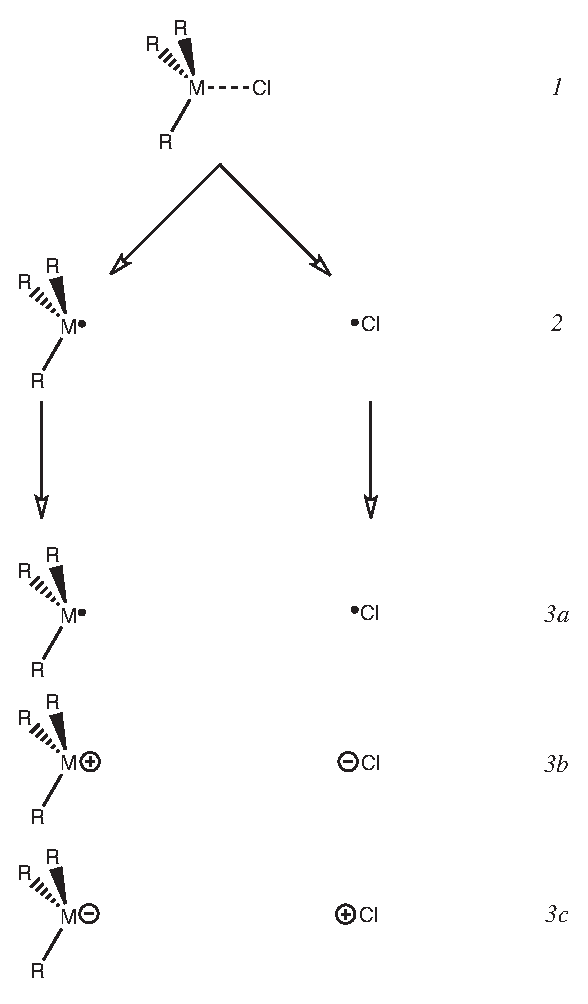
\includegraphics{dissociation/figures/scheme1.eps}
\end{center}
\caption{The three steps to generate dissociation curves: \textit{1.} Geometry optimization at fixed M--Cl (dashed) bonds. \textit{2.} Generation of start-up orbitals on radical fragments. \textit{3.} Valence Bond calculations on the three Lewis structures separately (\textit{3a}, \textit{3b} and \textit{3c}) and together (\textit{3a} + \textit{3b} + \textit{3c}).} 
\label{ch3.fig.scheme1}
\end{figure}
After these geometry optimizations start-up orbitals were generated on the R$_3$M$^{\bullet}$ and Cl$^{\bullet}$ fragments separately at the \mbox{RHF/6-31G*} level (step \textit{2} in Figure \ref{ch3.fig.scheme1}).  With these orbitals the Valence Bond wave functions containing the covalent (\textit{3a}) and both ionic (\textit{3b} and \textit{3c}) VB structures were constructed. The valence orbitals were subsequently optimized at the \mbox{VBSCF/6-31G*} level \cite{vbscf1,vbscf2}, while the core orbitals were frozen at their \mbox{RHF/6-31G*} levels.
Through the use of the local VBSCF model the valence orbitals were optimized on both the R$_3$M and Cl fragments separately; basis functions of the other fragment were not allowed to mix in, keeping the orbitals expressed in basis functions of a single fragment. All calculations were performed with TURTLE \cite{turtle} as implemented in GAMESS-UK \cite{gamess}.

\subsection{Results and Discussion}

The optimal M--Cl bond lengths ($R_\mathrm{eq}$) and the corresponding dissociation energies ($E_\mathrm{dis}^\mathrm{gas}$) are shown in Table \ref{ch3.tab.optimal}. $E_\mathrm{dis}^\mathrm{gas}$ is the difference between the lowest energy (at equilibrium) and the energy at 10 \AA. The optimal VB M--Cl bond lengths are obtained by a three-point fit through the three lowest points around the equilibrium. This is needed, because the GVB minimum is not exactly equal to the VBSCF minimum. Since the orbitals in VBSCF are kept localized on either of the two fragments, the minima differ slightly. With the fitted bond lengths additional VBSCF calculations have been performed from which the VB energy was used. Next to our $E_\mathrm{dis}^\mathrm{gas}$ values, the corresponding values from literature and experimental values \cite{lauvergnat,psu} are shown. In the last column, the charge-shift resonance energy ($RE_{CS}$ \cite{cs1}) is presented. This is the difference between the total energy and the energy of most stable structure at equilibrium distance. 
\begin{table}[hbtp]
\center
\caption{The VB dissociation energy $E_\mathrm{dis}^\mathrm{gas}$, literature data \cite{lauvergnat,psu}, optimal M--Cl bond lengths and the resonance energy for charge-shift bonds ($RE_{CS}$) \cite{cs1}. $^\mathrm{a}$ 404.2 kJ/mol is computed with VBSCF with delocalized orbitals that  are not restricted to either the chlorine, or the trimethylsilyl fragment.}  
\begin{tabular}{|l|c|c|c|c|c|}
\hline
Compound & \multicolumn{3}{c|}{$E_\mathrm{dis}^\mathrm{gas}$ (kJ/mol)} & $R_\mathrm{eq}$ (\AA) & $RE_{CS}$ \\
\hline
&\multicolumn{1}{c|}{this} & \multicolumn{1}{c|}{earlier} & \multicolumn{1}{c|}{exp.} & (M--Cl length) & (kJ/mol) \\
&\multicolumn{1}{c|}{work} & \multicolumn{1}{c|}{VB calculations} & \multicolumn{1}{c|}{} & & \\
\hline
CH$_3$Cl (\textbf{1})& 260.9 & 255.6 \cite{lauvergnat} & 365.3 \cite{lauvergnat} & 1.894 & 179.9\\
C(CH$_3$)$_3$Cl (\textbf{2}) & 251.3 & 245.6 \cite{psu} & 360.7 \cite{psu} & 1.935 & 183.6\\
SiH$_3$Cl (\textbf{3})& 335.5 & 331.1 \cite{lauvergnat} & 463.2 \cite{lauvergnat} & 2.154 & 266.4\\
Si(CH$_3$)$_3$Cl (\textbf{4}) & 371.5 & 404.2$^\mathrm{a}$ \cite{psu} & --- & 2.175 & 310.4\\
\hline
\end{tabular}
\label{ch3.tab.optimal}
\end{table}
Our calculated dissociation energies for \textbf{1}, \textbf{2} and \textbf{3} are in good agreement with earlier reported values at the VBSCF/6-31G* level of theory \cite{lauvergnat, psu}. As noted earlier, Lauvergnat \textit{et al.} \cite{lauvergnat} concluded that BOVB produces dissociation energies that are close to the experimental value, but that VBSCF calculations suffice to obtain qualitatively correct results.

\begin{figure}[hbtp]
\begin{center}
\includegraphics[scale=0.55]{dissociation/figures/ch3cl_g.eps}
\end{center}
\caption{The dissociation curve of chloromethane (CH$_3$Cl; \textbf{1}) in the gas phase. $E_\mathrm{tot}^\mathrm{gas}$ is the total VB energy. $E_\mathrm{cov}^\mathrm{gas}$ is the energy of structure \textbf{a} and $E_\mathrm{ion}^\mathrm{gas}$ is the energy of structure \textbf{b} separately. The minima are shown in parenthesis.}
\label{ch3.fig.ch3cl}
\end{figure}

For \textit{tert}-butylchloride (\textbf{2}) the dissociation energy is 9.6 kJ/mol lower than for chloromethane (\textbf{1}). For trimethylsilylchloride (\textbf{4}) it is 36.0 kJ/mol higher than for chlorosilane (\textbf{3}). Comparing the carbon compounds to the silicon ones, it can be seen that the silicon chlorine bond is much stronger than the carbon chlorine bond.

Regarding the charge-shift resonance energy ($RE_{CS}$), it is significantly higher for the silicon compounds (266.4 kJ/mol for \textbf{3} and 310.4 kJ/mol for \textbf{4}) than for the carbon analogues (179.9 kJ/mol for \textbf{1} and 183.6 kJ/mol for \textbf{2}).

The dissociation curves of \textbf{1}-\textbf{4} are shown in Figures \ref{ch3.fig.ch3cl}, \ref{ch3.fig.c4h9cl}, \ref{ch3.fig.sih3cl} and \ref{ch3.fig.c3h9sicl}. All Figures consist of three curves in the gas phase: the total VB energy ($E_\mathrm{tot}^\mathrm{gas}$), the energy of the covalent structure \textbf{3a} ($E_\mathrm{cov}^\mathrm{gas}$) and the energy of ionic structure \textbf{3b} ($E_\mathrm{ion}^\mathrm{gas}$), which corresponds to R$_3$M$^{+}$ and Cl$^{-}$. The curve for R$_3$M$^{-}$ and Cl$^{+}$ (the other ionic structure \textbf{3c}) has been omitted, since the energy for \textbf{3c} was \textit{ca.} 0.3 - 0.5 a.u. higher than for the other structures over the whole range. Hence, its contribution to the wave function proved to be small.

\begin{figure}[b]
\begin{center}
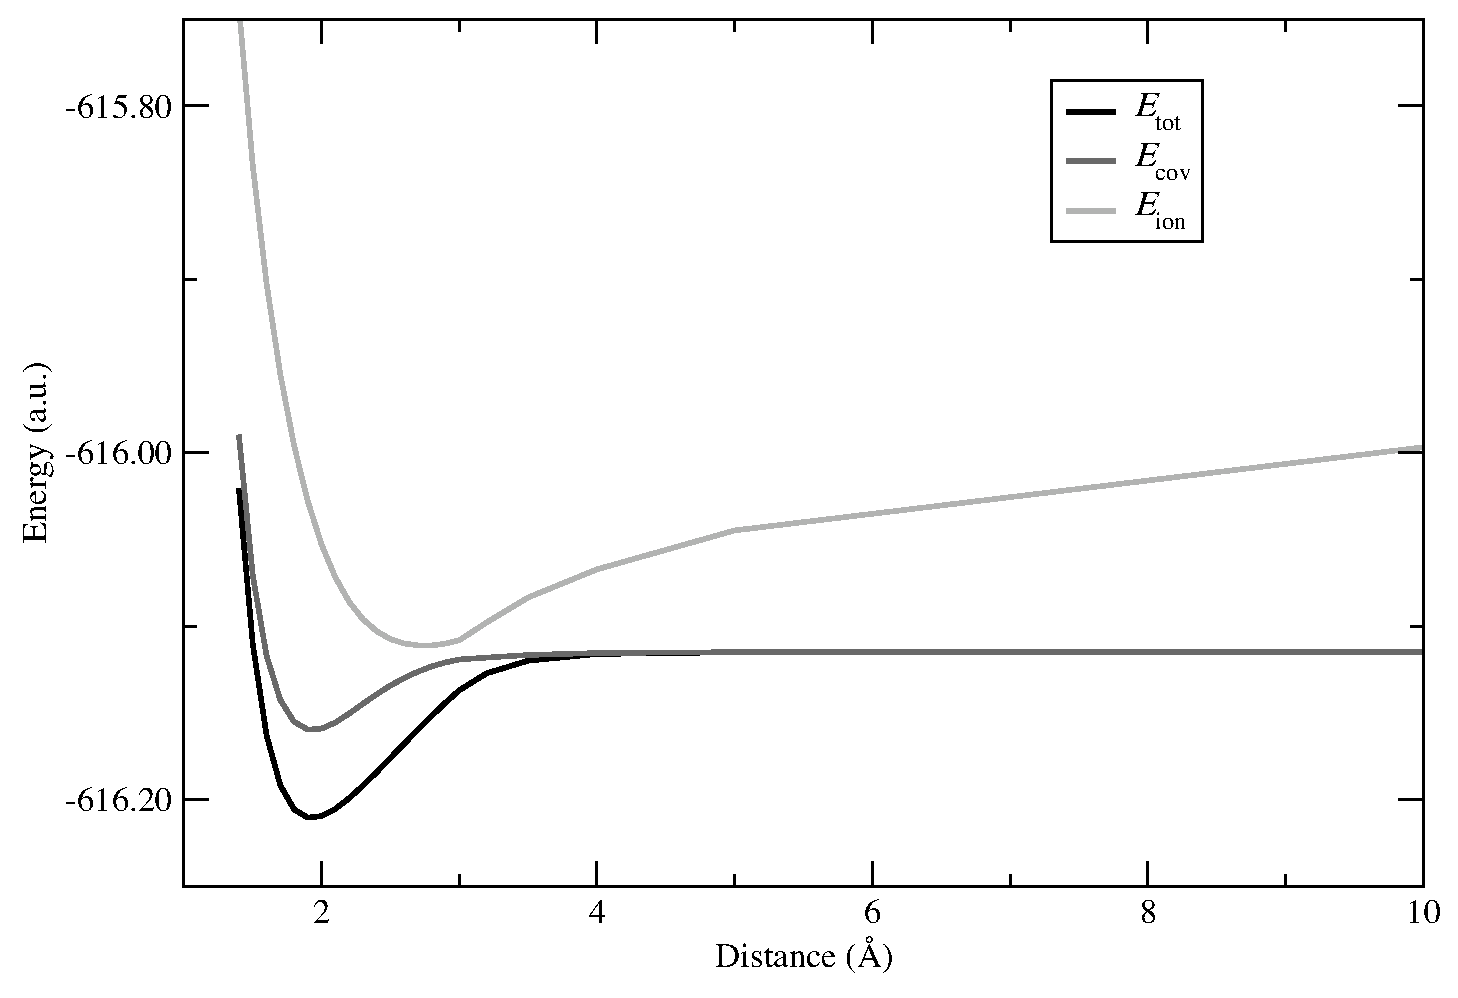
\includegraphics[scale=0.55]{dissociation/figures/c4h9cl_g.eps}
\end{center}
\caption{The dissociation curve of \textit{tert}-butylchloride (C(CH$_3$)$_3$Cl; \textbf{2}) in the gas phase. $E_\mathrm{tot}^\mathrm{gas}$ is the total VB energy. $E_\mathrm{cov}^\mathrm{gas}$ is the energy of structure \textbf{a} and $E_\mathrm{ion}^\mathrm{gas}$ is the energy of structure \textbf{b} separately. The minima are shown in parenthesis.}
\label{ch3.fig.c4h9cl}
\end{figure}

Chloromethane (\textbf{1}; Figure \ref{ch3.fig.ch3cl}) shows covalent bond character over the whole range.
\begin{figure}[t]
\begin{center}
\includegraphics[scale=0.55]{dissociation/figures/sih3cl_g.eps}
\end{center}
\caption{The dissociation curve of chlorosilane (SiH$_3$Cl; \textbf{3}) in the gas phase. $E_\mathrm{tot}^\mathrm{gas}$ is the total VB energy. $E_\mathrm{cov}^\mathrm{gas}$ is the energy of structure \textbf{a} and $E_\mathrm{ion}^\mathrm{gas}$ is the energy of structure \textbf{b} separately. The minima are shown in parenthesis.}
\label{ch3.fig.sih3cl}
\end{figure}
\begin{figure}[t]
\begin{center}
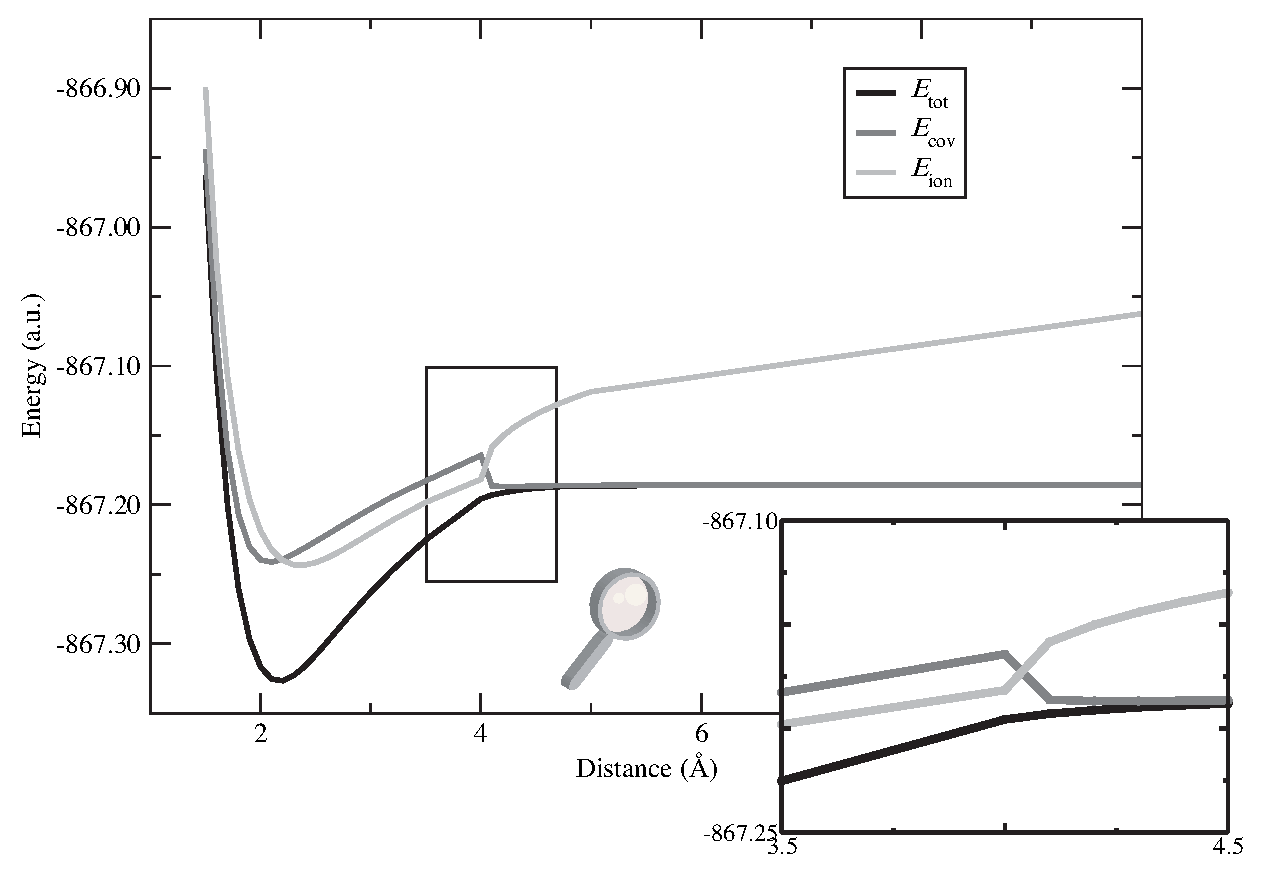
\includegraphics[scale=0.55]{dissociation/figures/c3h9sicl_g.eps}
\end{center}
\caption{The dissociation curve of trimethylsilylchloride (Si(CH$_3$)$_3$Cl; \textbf{4}) in the gas phase. $E_\mathrm{tot}^\mathrm{gas}$ is the total VB energy. $E_\mathrm{cov}^\mathrm{gas}$ is the energy of structure \textbf{a} and $E_\mathrm{ion}^\mathrm{gas}$ is the energy of structure \textbf{b} separately. The minima are shown in parenthesis.}
\label{ch3.fig.c3h9sicl}
\end{figure}
The weight of the covalent structure is 0.67 at equilibrium distance and higher for longer distances. The bond character for \textit{tert}-butylchloride (\textbf{2}; Figure \ref{ch3.fig.c4h9cl}) is also covalent, because the weight for the covalent structure is at least 0.66 over the whole range of the curve.
In the chlorosilane (\textbf{3}) case (Figure \ref{ch3.fig.sih3cl}) the bonding energy is 74.6 kJ/mol higher than in the chloromethane (\textbf{1}) case (Table \ref{ch3.tab.optimal}), indicating that the Si--Cl bond is much stronger than the C--Cl bond. 

For trimethylsilylchloride (\textbf{4}; Figure \ref{ch3.fig.c3h9sicl}) the Coulombic character is more pronounced. For distances from 2.0 to 4.1 \AA\  the ionic curve ($E_\mathrm{ion}^\mathrm{gas}$) lies below the covalent curve ($E_\mathrm{cov}^\mathrm{gas}$). The weight of the ionic structure is higher than that of the covalent structure between 2.3 and 4.1 \AA, which is in line with the expectation that this bond possesses a higher ionic character. Still, the bonds in trimethylsilylchloride (\textbf{4}) and NaCl are quite different, because for the NaCl ``molecule'' the ionic and total curve almost coincide, while for \textbf{4} this is not the case, although the ionic curve lies lower in energy than the covalent curve near the equilibrium distance. At large distance this situation is reversed (compare Figure \ref{ch3.fig.nacl_c} with Figure \ref{ch3.fig.c3h9sicl}). Regarding the shape of the curve, at the crossing of the ionic and covalent curves for \textbf{4} around 2.2 \AA\ the geometry does not change drastically. Therefore, this crossing is not accompanied by any kind of discontinuity in contrast to the crossing around 4.0 \AA\ (\textit{vide infra}). At distances shorter than the Si--Cl equilibrium bond distance the negative charge cloud on the chlorine atom starts to overlap with the positive Si(CH$_3$)$_3$ fragment. This stabilizes the neutral covalent structure, which results in a lower value for $E_\mathrm{cov}^\mathrm{gas}$ than for $E_\mathrm{ion}^\mathrm{gas}$. 

Regarding the shape, the total energy ($E_\mathrm{tot}^\mathrm{gas}$) for \textbf{4} increases more gradually than for \textbf{2}, showing more Coulombic character. This is because from the equilibrium distance to the crossing, the ionic curve lies below the covalent curve, similar to the NaCl curves. In the other cases the covalent curve lies below the ionic curve over the whole range. An analysis of the Mulliken population on the chlorine and carbon/silicon atoms corroborates the Coulombic shape for \textbf{4}: the population on chlorine ($Z$=17) is 17.24 for \textbf{2} and 17.51 for \textbf{4}. While the population on carbon ($Z$=6) is 6.03 for \textbf{2}, the population on silicon ($Z$=14) for \textbf{4} is only 12.88. This indicates that the methyl groups have a slight electron donating character in \textit{tert}-butyl, while in the trimethylsilyl case they have an electron withdrawing effect. The extra Coulombic attraction results in a (much) stronger bond for \textbf{4} (371.5 kJ/mol) than for \textbf{2} (251.3 kJ/mol). 

An intriguing feature seen in Figures \ref{ch3.fig.c4h9cl} and \ref{ch3.fig.c3h9sicl} is the abrupt rise in energy of the ionic curve at around 3.0 \AA\ for \textbf{2} and around 4.0 \AA\ for \textbf{4} and the abrupt fall in energy of the covalent curve at the same points. In contrast, the total energy rises modestly with increasing bond distance at those points. To understand this behavior, one has to examine the underlying geometry of the molecules at these points. For \textbf{4}, the effect is most pronounced and will be discussed here. For \textbf{2}, the same reasoning can be applied. The reason for the crossing of the covalent and ionic curves is that the geometry for \textbf{4} at 4.0 \AA\ is completely different from that at 4.1 \AA. At 4.0 \AA\ the bond is ionic and hence the trimethylsilyl fragment is cation-like in which the silicon and the three carbon atoms are nearly coplanar after geometry optimization (Figure \ref{ch3.fig.crossing}(a)). This geometry is unfavorable for the covalent structure alone, reflected in the high energy.  In contrast, at 4.1 \AA\  the bond is covalent and the trimethylsilyl is radical-like, in which the silicon and the three carbon atoms form a tetrahedral structure (Figure \ref{ch3.fig.crossing}(b)), resulting in a lower covalent structure energy. 
\begin{figure}[hbtp]
\center
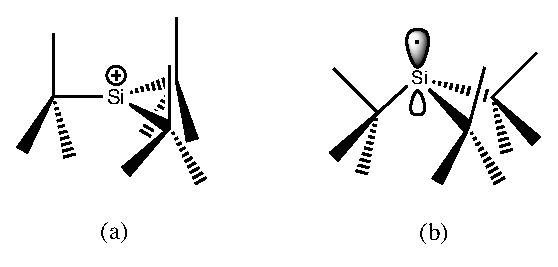
\includegraphics[scale=1.0]{dissociation/figures/crossing.eps}
\caption{The cation-like structure with coplanar silicon (M=Si), carbon (M=C)) and methyl carbon atoms (a) and the radical-like tetrahedral structure (b).}
\label{ch3.fig.crossing}
\end{figure}
Note that the total energy curve ($E_\mathrm{tot}^\mathrm{gas}$) does not show any irregularities.  The wave function changes drastically in character at this point. This compound follows the dissociation path of the ionic structure at short distances and that of the covalent structure at longer distances. 

A comparison of the hydrogen and methyl substituted molecules suggests that methyl substitution has an energy lowering effect on the $E_\mathrm{ion}^\mathrm{gas}$ with respect to $E_\mathrm{cov}^\mathrm{gas}$. In the silicon case (\textbf{4}), the ionic curve even lies below the covalent curve between 2.3 and 4.1 \AA.

\section{\label{ch3.sec.solv}Solvation Effects}

\subsection{Computational Methods}

In the Polarizable Continuum Model (PCM) the solvent is represented as a homogeneous medium that is characterized by its dielectric constant. No further explicit molecular interactions between the solvent molecules and the solute are taken into account. For example, hydrogen-bond formation is absent. For the research presented here, the VB module TURTLE and the PCM algorithm in GAMESS-UK were linked.

The PCM model requires a number of parameters. First of all, a dielectric constant, for which the value of water (H$_2$O, $\epsilon$=78.5) was chosen. The second parameter is the interspacing of the point charges, which was set to 30.0\degrees. The last set of parameters contains the dimensions of the spheres around the atoms. As an estimate for these the van der Waals radii \cite{bondi} were taken, scaled by 1.20 (being the average of the optimal 1.15 for ions and 1.25 for neutral atoms \cite{scaling}) resulting in 1.44 \AA\  for hydrogen, 2.16 \AA\  for carbon, 2.69 \AA\ for silicon and 2.10 \AA\ for chlorine and chloride.

For each compound two points on the potential energy curve were analyzed with VBPCM. One calculation was performed at the equilibrium distance and one at large distance (10 \AA). For the point at equilibrium distance the gas phase optimized geometries were taken. For the point at large distance the R$_3$M-fragments were optimized in two ways: as the covalent structure (a geometry optimization on the radical R$_3$M$^\bullet$-fragments) and as the ionic structure (a geometry optimization on the R$_3$M$^{+}$-fragments). Subsequently, the chlorine atoms were added to the R$_3$M-fragments at a distance of 10 \AA. 

\subsection{Results and Discussion}

In Table \ref{ch3.tab.solution} the VBPCM values are presented for the equilibrium distance ($E_\mathrm{R_{3}M-Cl}^\mathrm{solv}$) and for both neutrally and ionically optimized geometries at large distance (10 \AA), $E_\mathrm{R_{3}M^\bullet Cl^\bullet}^\mathrm{solv}$ and $E_\mathrm{R_{3}M^{+} Cl^{-}}^\mathrm{solv}$ respectively. Besides, the dissociation energy in the gas phase ($E_\mathrm{dis}^\mathrm{gas}$) and in solution ($E_\mathrm{dis}^\mathrm{solv}$) are shown in the last two columns.
\begin{table}[htp]
\center
\caption{The VBPCM energy at equilibrium distance ($E_\mathrm{R_{3}M-Cl}^\mathrm{solv}$), the VBPCM energies on the neutrally ($E_\mathrm{R_{3}M^\bullet Cl^\bullet}^\mathrm{solv}$) and ionically ($E_\mathrm{R_{3}M^{+} Cl^{-}}^\mathrm{solv}$) optimized geometries at long distance (10 \AA), and the dissociation energy ($E_\mathrm{dis}^\mathrm{solv}$), being the difference between the most stable long distance geometry (\textit{italics}) and the energy at equilibrium distance ($R_\mathrm{eq}$). The last column contains the dissociation energies from Table \ref{ch3.tab.optimal}. Energy values are in atomic units, except $E_\mathrm{dis}^\mathrm{solv}$ and $E_\mathrm{dis}^\mathrm{gas}$, which are in kJ/mol.}
\begin{tabular}{|l|c|c|c|c|c|}
\hline
\textbf{Compound} & $E_\mathrm{R_{3}M-Cl}^\mathrm{solv}$ ($E_{\mathrm{h}}$) & $E_\mathrm{R_{3}M^\bullet Cl^\bullet}^\mathrm{solv}$ ($E_{\mathrm{h}}$) & $E_\mathrm{R_{3}M^{+} Cl^{-}}^\mathrm{solv}$ ($E_{\mathrm{h}}$) & $E_\mathrm{dis}^\mathrm{solv}$&
$E_\mathrm{dis}^\mathrm{gas}$\\
\hline
CH$_3$Cl (\textbf{1})& --499.102862 & \textit{--499.000733} & --498.984663 & 268.1 & 260.9 \\
C(CH$_3$)$_3$Cl (\textbf{2})& --616.215591 & --616.116711 & \textit{--616.165131} & 132.5 & 251.3 \\
SiH$_3$Cl (\textbf{3})& --750.179837 & --750.049132 & \textit{--750.065038} &  301.4 & 335.5 \\
Si(CH$_3$)$_3$Cl (\textbf{4})& --867.333824 & --867.187477 & \textit{--867.248816} & 223.2 & 371.5 \\
\hline
\end{tabular}
\label{ch3.tab.solution}
\end{table} 

The ionic structures are more stabilized by the polar solvent than the covalent structures. At large distances the ionic structure has a lower energy ($E_\mathrm{ion}^\mathrm{solv}$) for \textbf{2}, \textbf{3} and \textbf{4} in the polar medium. This indicates that for these molecules the dissociation changes from homolytic to heterolytic with PCM in the presence of a polar solvent (here H$_2$O). For \textbf{1}, which contains the least polar bond, the ionic structure is stabilized, however, not enough to change the dissociation to heterolytic in the solvent model.

For both the methyl substituted compounds, the lowering in dissociation energy in solution compared to the gas phase is standing out, most remarkable for \textbf{2}. While in the gas phase the dissociation energy of \textbf{4} is higher than for \textbf{3}, in solution the situation is reversed. The reason for this is the stabilization of the planar structure of the \textit{tert}-butyl and \textit{tert}-silyl  (Figure \ref{ch3.fig.crossing}(a)) cations in solution compared to the umbrella shaped radical fragment in the gas phase (Figure \ref{ch3.fig.crossing}(b)).

\section{The Frozen Orbital Approximation}

Upon comparing the ionic and covalent curves for \textit{tert}-butylchloride (\textbf{2}) shown in Figure \ref{ch3.fig.c4h9cl} with those in the article by Song \textit{et al.} \cite{song}, we have noted that in the article by Song the ionic and covalent curves cross twice, while in our curves there is no crossing between the two curves. One difference between both calculations appeared to be the use of frozen orbitals for the C--H bonds by Song, while we optimized those with the other orbitals. Therefore, the impact of the freezing of orbitals will be investigated here for \textbf{2}.

\subsection{Computational Methods}

Two points on the C--Cl reaction coordinate were taken, one at equilibrium distance and one at \mbox{10 \AA}. For the point at 10 \AA, the umbrella shaped \textit{tert}-butyl fragment was used for the gas phase (Figure \ref{ch3.fig.crossing}(b)), while the planar shaped fragment was used for in solution (Figure \ref{ch3.fig.crossing}(a)). The start-up orbitals for both fragments were generated with a RHF wave function with the 6-31G* basis set. For each point two sets of RHF start-up orbitals were generated: \textbf{I}) for the neutral fragments (CH$_3$)$_3$C$^\bullet$ and Cl$^\bullet$ (homolytic dissociation) and \textbf{II}) for the ions, (CH$_3$)$_3$C$^{+}$ and Cl$^{-}$ (heterolytic dissociation). Subsequently, the orbitals on the (CH$_3$)$_3$C$^\bullet$ and (CH$_3$)$_3$C$^{+}$ fragments were localized using the Foster-Boys algorithm \cite{foster}. The localized orbitals describing the inner-shells and C--H bonds were frozen during the subsequent VB calculations, as were the core orbitals of chlorine and carbon. For the PCM solvation model the same parameters as in Section \ref{ch3.sec.solv} were used.

\subsection{\label{ch3.sec.res.freez}Results and Discussion}

The total VB energies for calculations with start-up sets \textbf{I} and \textbf{II}, together with the VB energies from Section \ref{ch3.sec.solv} ($E_\mathrm{free}$) are given in Table \ref{ch3.tab.frozen}. 
\begin{table}[htp]
\center
\caption{VB energies without frozen C--H bonds ($E_\mathrm{free}$), with frozen C--H bonds based on
start-up set \textbf{I} ($E_\mathrm{froz-\textbf{I}}$) and with frozen C--H bonds based on start-up set \textbf{II}
($E_\mathrm{froz-\textbf{II}}$) at equilibrium distance ($R_{eq}$) and at 10.0 \AA\ ($R_{10.0 \text{\AA}}$),
both in the gas phase and in solution (in $E_\mathrm{h}$). The dissociation energy in gas phase ($E_\mathrm{dis}^\mathrm{gas}$) and in solution ($E_\mathrm{dis}^\mathrm{solv}$), both in kJ/mol.}
\center
\begin{tabular}{|c|cc|cc|c|c|}
\hline
&\multicolumn{2}{c|}{$R_{eq}$}&\multicolumn{2}{c|}{$R_{10.0 \text{\AA}}$} & $E_\mathrm{dis}^\mathrm{gas}$ & $E_\mathrm{dis}^\mathrm{solv}$ \\
\textbf{Energy} & gas & solv & gas & solv &  & \\
\hline
$E_\mathrm{free}$ & {--616.210349} & {--616.215591} & {--616.114616} & {--616.165131} & 251.3 & 132.5 \\
$E_\mathrm{froz-\textbf{I}}$& {--616.208752} & {--616.213543} & {--616.114616} & {--616.132413} & 247.2 &  213.0 \\
$E_\mathrm{froz-\textbf{II}}$& {--616.186693} & {--616.194963} & {--616.080074} & {--616.164974} & 279.9 & 78.7\\
\hline
\end{tabular}
\label{ch3.tab.frozen}
\end{table}

The values on the first row of the table correspond to those presented earlier in this chapter. The energy value at 10 \AA\ in the gas phase is equal to the corresponding energy value with the freely optimized orbitals ($E_\mathrm{froz-\textbf{I}}^{R_{10.0 \text{\AA}},\mathrm{gas}}$ = $E_\mathrm{free}^{R_{10.0 \text{\AA}},\mathrm{gas}}$ = {--616.114616}). The reason is that at 10 \AA\ both fragments are so far apart that they can be considered as two separate radicals. Since the orbitals are optimized for radicals, they do not need to change much and hence, frozen or not, they are already optimal from the start. At equilibrium distance,  both fragments are closer and hence, the free C--H orbitals are adopted to the presence of the chlorine atom ($E_\mathrm{free}^{R_{eq},\mathrm{gas}}$ = {--616.210349}, opposed to $E_\mathrm{froz-\textbf{I}}^{R_{eq},\mathrm{gas}}$ = {--616.208752}). In solution, the difference at equilibrium distance is smaller than in the gas phase ($E_\mathrm{free}^{R_{eq},\mathrm{solv}}$ = {--616.215591}, compared to $E_\mathrm{froz-\textbf{I}}^{R_{eq},\mathrm{solv}}$ = {--616.213543}). At 10.0 \AA\ the difference is large, $E_\mathrm{free}^{R_{10.0 \text{\AA}},\mathrm{solv}}$ = {--616.165131}, compared to $E_\mathrm{froz-\textbf{I}}^{R_{10.0 \text{\AA}},\mathrm{solv}}$ = {--616.132413}. Since C(CH$_3$)$_3$Cl dissociates to ions in solution, the start up with frozen orbitals for radicals appears to be unfavorable. The dissociation energy in solution ($E_\mathrm{dis}^\mathrm{solv}$) goes up from 132.5 kJ/mol for free orbitals to 213.0 kJ/mol for frozen orbitals started with radicals.

The frozen orbitals for ionic fragments result in much higher energies at equilibrium, both in the gas phase as in solution, \textit{viz.} $E_\mathrm{froz-\textbf{II}}^{R_{eq},\mathrm{gas}}$ = {--616.186693} and $E_\mathrm{froz-\textbf{II}}^{R_{eq},\mathrm{solv}}$ = {--616.194963}, compared to the corresponding values for $E_\mathrm{free}$. Also the energy for the gas phase at 10 \AA\ is much higher than for free orbitals, $E_\mathrm{froz-\textbf{II}}^{R_{10.0 \text{\AA}},\mathrm{gas}}$ = {--616.080074} compared to $E_\mathrm{free}^{R_{10.0 \text{\AA}},\mathrm{gas}}$ = {--616.114616}. The only energy value for ionically optimized start up orbitals that is close to the corresponding value for free orbitals, is the one in solution at 10 \AA, $E_\mathrm{froz-\textbf{II}}^{R_{10.0 \text{\AA}},\mathrm{solv}}$ = {--616.164974} compared to $E_\mathrm{free}^{R_{10.0 \text{\AA}},\mathrm{solv}}$ = {--616.165131}. This can easily be explained. Since \textbf{2} dissociates to ions in solution, the ionic C--H start up orbitals, frozen at the RHF level, are close to the optimal ones obtained with free optimization.

This indicates that the way the frozen C--H orbitals are optimized, \textit{i.e.} for the \textit{tert}-butyl radical and the \textit{tert}-butyl cation, has a non negligible influence on the wave function and hence on the dissociation energy. Therefore, the C--H bonds are not mere spectators: they play a vital role in the dissociation process. In the next section, the interaction of the C--H bonds with the central carbon atom, linked to hyperconjugation \cite{march,mcmurry}, is investigated in more detail.
 
\subsection{Hyperconjugation}

When the C--H bond orbitals are frozen, the interactions between them and the $p$ orbital on the central carbon atom are absent in the wave function (Figure \ref{ch3.fig.hyperconjugation}).
\begin{figure}[ht]
\center
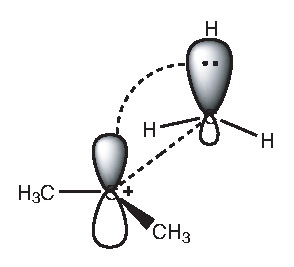
\includegraphics{dissociation/figures/hyperconj.eps}
\caption{The hyperconjugation effect: the $p$ orbital on the central carbon atom has interaction with the neighboring C--H orbital.}
\label{ch3.fig.hyperconjugation}
\end{figure}

Hyperconjugation can be included or excluded from the Valence Bond wave function by applying appropriate restrictions during orbital optimization.  Calculations on the constrained $C_\mathrm{3h}$ geometries (Figure \ref{ch3.fig.c3h}) of the \textit{tert}-butyl cation, the trimethylsilylcation, and of their radicals have been performed in which the empty/singly occupied $p$ orbital on the central carbon/silicon atom is constrained to remain strictly atomic in nature, thereby excluding the effect of hyperconjugation.
\begin{figure}[ht]
\center
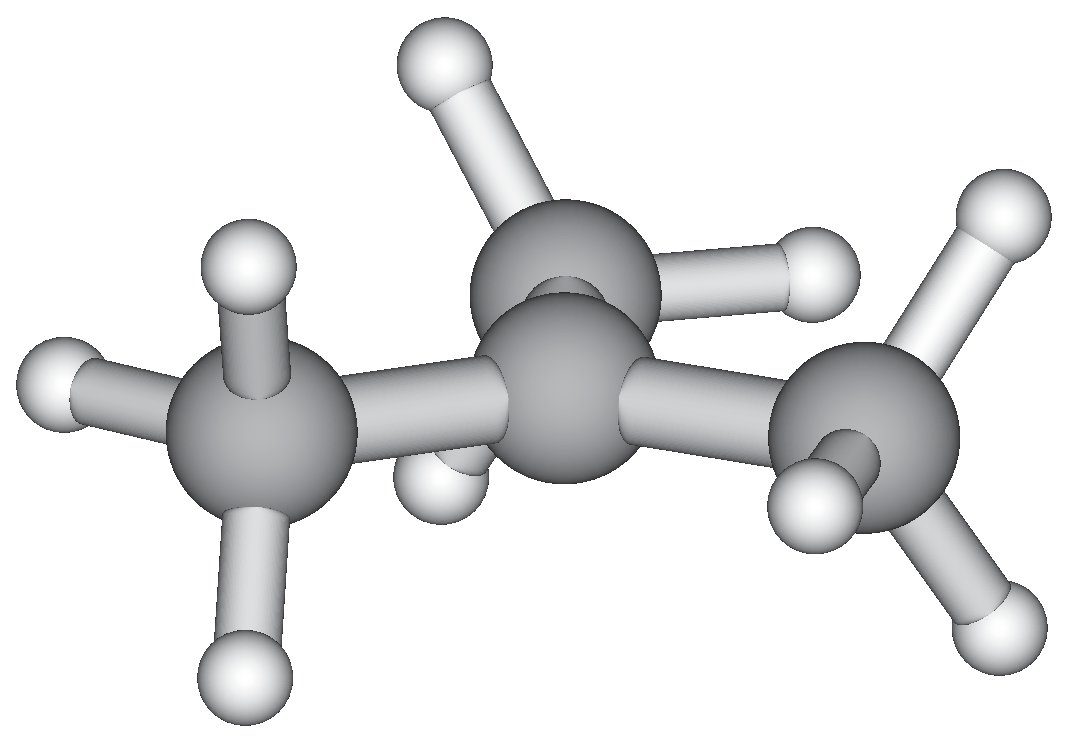
\includegraphics{dissociation/figures/c3h.eps}
\caption{Schematic representation of the \textit{tert}-butyl fragment in $C_\mathrm{3h}$ symmetry.}
\label{ch3.fig.c3h}
\end{figure}
A wave function that consists of several blocks of localized (orthogonal) orbitals per block is called a Block Localized Wave Function (BLW) \cite{blw}. These orbital blocks are not (necessarily) orthogonal to each other. Comparison of the energy obtained with this constrained wave function with that by an unconstrained calculation  (non localized Hartree-Fock in this case) yields an estimate of the magnitude of the stabilization by hyperconjugation for the respective cations and radicals. 

\begin{table}[htp]
\center
\caption{Energies of the cation and radical of \textit{tert}-butyl and of the cation and the radical of trimethylsilyl obtained using a constrained VB wave function with a strictly atomic $p$ orbital ($E_\mathrm{VB-res}$) in the first column. The second column shows the Hartree-Fock energies ($E_\mathrm{HF}$) and the third column contains their difference $\Delta E$ (in kJ/mol).}
\label{ch3.tab.hyp}
\begin{tabular}{|c|c|c|c|}
\hline
\textbf{Compound} & $E_\mathrm{VB-res}$ ($E_{\mathrm{h}}$) &$E_\mathrm{HF}$ ($E_{\mathrm{h}}$)& $\Delta E$ (kJ/mol)  \\
\hline
\textit{tert}-butyl cation & -156.399322 &-156.442412&113.1  \\
\textit{tert}-butyl radical & -156.630889 &-156.661317&79.9 \\
trimethylsilyl cation & -407.509449&-407.526979&46.0 \\
trimethylsilyl radical &-407.687692&-407.704949&45.3 \\
\hline
\end{tabular}
\end{table}

From a survey of the data in Table \ref{ch3.tab.hyp} follows that the stabilization obtained for the cation and the radical by mixing of the C--H bonds with the central $p$ orbital of carbon is considerable, and substantially larger in the case of the cation than for the radical.  This  corroborates that the \textit{tert}-butyl C--H bonds of the cation differ markedly from that of the radical, as was already noted from the calculations with the different sets of frozen orbitals.  Note that for the \textit{tert}-butyl radical, the equilibrium geometry will deviate from $C_\mathrm{3h}$ symmetry, and the central $p$ orbital will rehybridize.  As a consequence of the geometric distortion and their rehybridization, the overlap between the central carbon $p$ orbital and the C--H bonds will be smaller, thus the above mentioned stabilization of 79.9 kJ/mol is an upper bound.  These calculations provide strong evidence for the large stabilizing effect that hyperconjugation exerts on the central carbon atom, and as a consequence, freezing these orbitals to describe two different reaction pathways may lead to substantial errors.  Furthermore, hyperconjugation is only important in the dissociated fragments.

For the silicon case, although a stabilization is found, it is considerably smaller than for the carbon analogue.  The trimethylsilyl cation and radical are equally stabilized.  The smaller stabilization of the trimethylsilyl fragment with respect to their carbon analogues is attributed to the more electropositive nature of silicon. Thus, hyperconjugation is less important for trimethylsilyl compounds than for the carbon analogues.

\section{Conclusions}

Both the weights and the similarity of the forms of the dissociation curves to that of H$_2$ for the C--Cl bonds of \textbf{1} and \textbf{2}, indicate that these bonds are mainly covalent.  The Si--Cl bonds are more ``Coulombic'' in nature; the shape of the dissociation curves is resembling the one of NaCl. Because neither the energy of the covalent structure nor of the ionic structure coincides with the total energy, these bonds are categorized as charge-shift bonds. The abrupt rise in the ionic curve and the steep drop in the covalent curve in the dissociation curves for \textbf{2} and \textbf{4} are caused by the dramatic change in geometry, due to the change in character from ionic to covalent of the wave function. The reaction paths of the single structures in the wave function differ from that of the total three-structure wave function.

Substitution of hydrogen for methyl groups does not change the C/Si--Cl bond directly, but the methyl groups exert an effect on the dissociated fragments through hyperconjugation.  The C--H bonds participate in the reaction.  Change to a medium that mimics a polar solvent (water) stabilizes the ionic curve, and may therefore change the dissociation from homo- to heterolytic, if the resulting cation is also stabilized by its electropositiveness or hyperconjugation.
 
\section*{Acknowledgement}

Part of this research was conducted in the Laboratoire de Chimie Physique, Paris XI (France) and was funded by the European Union (a Marie Curie host fellowship) and the Netherlands Organization for Scientific Research (NWO).

\bibliography{dissociation}
\bibliographystyle{../main/achemso}
